\onecolumngrid

\begin{figure}[H]
    \centering
    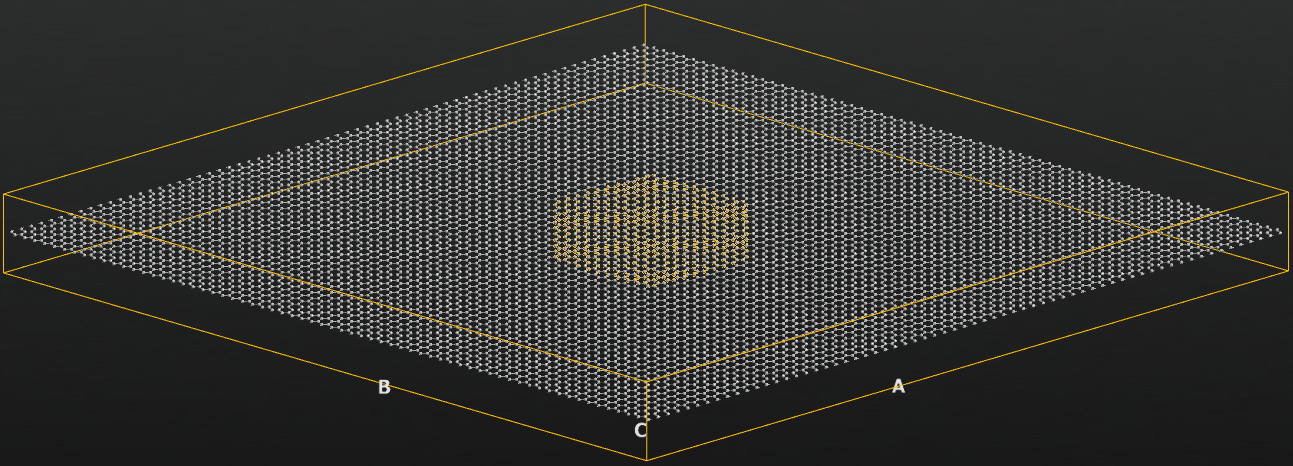
\includegraphics[width=\columnwidth]{Figures/NanoLayer5nm.png}
    \caption{A snapshot from ATK\cite{QuantumWise} showing how the clamped system looks like when at rest. The hexagon in the middle is marked with tags and is the only part of the sheet that is not constrained i.e. the free standing membrane.}
    \label{fig:clamped}
\vspace{12em}
    \centering
    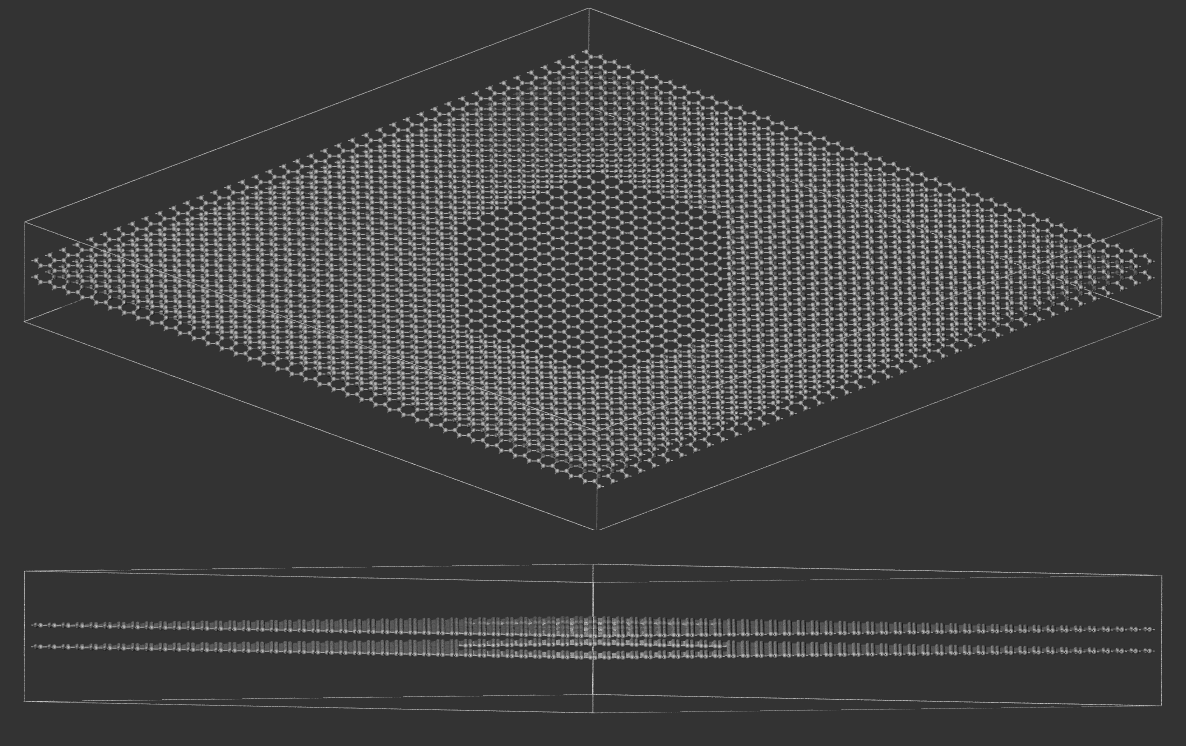
\includegraphics[width=\columnwidth]{Figures/DoubleMembrane.png}
\caption{The picture on top shows the two layer system from above. The one on bottom shows the system from the side. Both snapshots have been taken in ATK\cite{QuantumWise}.}
\label{interlayersys}
\end{figure}
\twocolumngrid
